\documentclass[]{book}
\usepackage{lmodern}
\usepackage{amssymb,amsmath}
\usepackage{ifxetex,ifluatex}
\usepackage{fixltx2e} % provides \textsubscript
\ifnum 0\ifxetex 1\fi\ifluatex 1\fi=0 % if pdftex
  \usepackage[T1]{fontenc}
  \usepackage[utf8]{inputenc}
\else % if luatex or xelatex
  \ifxetex
    \usepackage{mathspec}
  \else
    \usepackage{fontspec}
  \fi
  \defaultfontfeatures{Ligatures=TeX,Scale=MatchLowercase}
\fi
% use upquote if available, for straight quotes in verbatim environments
\IfFileExists{upquote.sty}{\usepackage{upquote}}{}
% use microtype if available
\IfFileExists{microtype.sty}{%
\usepackage{microtype}
\UseMicrotypeSet[protrusion]{basicmath} % disable protrusion for tt fonts
}{}
\usepackage[margin=1in]{geometry}
\usepackage{hyperref}
\hypersetup{unicode=true,
            pdftitle={Answering questions with data: Lab Manual},
            pdfauthor={Matthew J. C. Crump; Anajali Krishnan; Stephen Volz; Alla Chavarga; Jeffrey Suzuki},
            pdfborder={0 0 0},
            breaklinks=true}
\urlstyle{same}  % don't use monospace font for urls
\usepackage{natbib}
\bibliographystyle{apalike}
\usepackage{color}
\usepackage{fancyvrb}
\newcommand{\VerbBar}{|}
\newcommand{\VERB}{\Verb[commandchars=\\\{\}]}
\DefineVerbatimEnvironment{Highlighting}{Verbatim}{commandchars=\\\{\}}
% Add ',fontsize=\small' for more characters per line
\usepackage{framed}
\definecolor{shadecolor}{RGB}{248,248,248}
\newenvironment{Shaded}{\begin{snugshade}}{\end{snugshade}}
\newcommand{\KeywordTok}[1]{\textcolor[rgb]{0.13,0.29,0.53}{\textbf{{#1}}}}
\newcommand{\DataTypeTok}[1]{\textcolor[rgb]{0.13,0.29,0.53}{{#1}}}
\newcommand{\DecValTok}[1]{\textcolor[rgb]{0.00,0.00,0.81}{{#1}}}
\newcommand{\BaseNTok}[1]{\textcolor[rgb]{0.00,0.00,0.81}{{#1}}}
\newcommand{\FloatTok}[1]{\textcolor[rgb]{0.00,0.00,0.81}{{#1}}}
\newcommand{\ConstantTok}[1]{\textcolor[rgb]{0.00,0.00,0.00}{{#1}}}
\newcommand{\CharTok}[1]{\textcolor[rgb]{0.31,0.60,0.02}{{#1}}}
\newcommand{\SpecialCharTok}[1]{\textcolor[rgb]{0.00,0.00,0.00}{{#1}}}
\newcommand{\StringTok}[1]{\textcolor[rgb]{0.31,0.60,0.02}{{#1}}}
\newcommand{\VerbatimStringTok}[1]{\textcolor[rgb]{0.31,0.60,0.02}{{#1}}}
\newcommand{\SpecialStringTok}[1]{\textcolor[rgb]{0.31,0.60,0.02}{{#1}}}
\newcommand{\ImportTok}[1]{{#1}}
\newcommand{\CommentTok}[1]{\textcolor[rgb]{0.56,0.35,0.01}{\textit{{#1}}}}
\newcommand{\DocumentationTok}[1]{\textcolor[rgb]{0.56,0.35,0.01}{\textbf{\textit{{#1}}}}}
\newcommand{\AnnotationTok}[1]{\textcolor[rgb]{0.56,0.35,0.01}{\textbf{\textit{{#1}}}}}
\newcommand{\CommentVarTok}[1]{\textcolor[rgb]{0.56,0.35,0.01}{\textbf{\textit{{#1}}}}}
\newcommand{\OtherTok}[1]{\textcolor[rgb]{0.56,0.35,0.01}{{#1}}}
\newcommand{\FunctionTok}[1]{\textcolor[rgb]{0.00,0.00,0.00}{{#1}}}
\newcommand{\VariableTok}[1]{\textcolor[rgb]{0.00,0.00,0.00}{{#1}}}
\newcommand{\ControlFlowTok}[1]{\textcolor[rgb]{0.13,0.29,0.53}{\textbf{{#1}}}}
\newcommand{\OperatorTok}[1]{\textcolor[rgb]{0.81,0.36,0.00}{\textbf{{#1}}}}
\newcommand{\BuiltInTok}[1]{{#1}}
\newcommand{\ExtensionTok}[1]{{#1}}
\newcommand{\PreprocessorTok}[1]{\textcolor[rgb]{0.56,0.35,0.01}{\textit{{#1}}}}
\newcommand{\AttributeTok}[1]{\textcolor[rgb]{0.77,0.63,0.00}{{#1}}}
\newcommand{\RegionMarkerTok}[1]{{#1}}
\newcommand{\InformationTok}[1]{\textcolor[rgb]{0.56,0.35,0.01}{\textbf{\textit{{#1}}}}}
\newcommand{\WarningTok}[1]{\textcolor[rgb]{0.56,0.35,0.01}{\textbf{\textit{{#1}}}}}
\newcommand{\AlertTok}[1]{\textcolor[rgb]{0.94,0.16,0.16}{{#1}}}
\newcommand{\ErrorTok}[1]{\textcolor[rgb]{0.64,0.00,0.00}{\textbf{{#1}}}}
\newcommand{\NormalTok}[1]{{#1}}
\usepackage{longtable,booktabs}
\usepackage{graphicx,grffile}
\makeatletter
\def\maxwidth{\ifdim\Gin@nat@width>\linewidth\linewidth\else\Gin@nat@width\fi}
\def\maxheight{\ifdim\Gin@nat@height>\textheight\textheight\else\Gin@nat@height\fi}
\makeatother
% Scale images if necessary, so that they will not overflow the page
% margins by default, and it is still possible to overwrite the defaults
% using explicit options in \includegraphics[width, height, ...]{}
\setkeys{Gin}{width=\maxwidth,height=\maxheight,keepaspectratio}
\IfFileExists{parskip.sty}{%
\usepackage{parskip}
}{% else
\setlength{\parindent}{0pt}
\setlength{\parskip}{6pt plus 2pt minus 1pt}
}
\setlength{\emergencystretch}{3em}  % prevent overfull lines
\providecommand{\tightlist}{%
  \setlength{\itemsep}{0pt}\setlength{\parskip}{0pt}}
\setcounter{secnumdepth}{5}
% Redefines (sub)paragraphs to behave more like sections
\ifx\paragraph\undefined\else
\let\oldparagraph\paragraph
\renewcommand{\paragraph}[1]{\oldparagraph{#1}\mbox{}}
\fi
\ifx\subparagraph\undefined\else
\let\oldsubparagraph\subparagraph
\renewcommand{\subparagraph}[1]{\oldsubparagraph{#1}\mbox{}}
\fi

%%% Use protect on footnotes to avoid problems with footnotes in titles
\let\rmarkdownfootnote\footnote%
\def\footnote{\protect\rmarkdownfootnote}

%%% Change title format to be more compact
\usepackage{titling}

% Create subtitle command for use in maketitle
\newcommand{\subtitle}[1]{
  \posttitle{
    \begin{center}\large#1\end{center}
    }
}

\setlength{\droptitle}{-2em}
  \title{Answering questions with data: Lab Manual}
  \pretitle{\vspace{\droptitle}\centering\huge}
  \posttitle{\par}
  \author{Matthew J. C. Crump \\ Anajali Krishnan \\ Stephen Volz \\ Alla Chavarga \\ Jeffrey Suzuki}
  \preauthor{\centering\large\emph}
  \postauthor{\par}
  \predate{\centering\large\emph}
  \postdate{\par}
  \date{2018-07-19}

\usepackage{booktabs}
\usepackage{amsthm}
\makeatletter
\def\thm@space@setup{%
  \thm@preskip=8pt plus 2pt minus 4pt
  \thm@postskip=\thm@preskip
}
\makeatother

\usepackage{amsthm}
\newtheorem{theorem}{Theorem}[chapter]
\newtheorem{lemma}{Lemma}[chapter]
\theoremstyle{definition}
\newtheorem{definition}{Definition}[chapter]
\newtheorem{corollary}{Corollary}[chapter]
\newtheorem{proposition}{Proposition}[chapter]
\theoremstyle{definition}
\newtheorem{example}{Example}[chapter]
\theoremstyle{definition}
\newtheorem{exercise}{Exercise}[chapter]
\theoremstyle{remark}
\newtheorem*{remark}{Remark}
\newtheorem*{solution}{Solution}
\begin{document}
\maketitle

{
\setcounter{tocdepth}{1}
\tableofcontents
}
\chapter*{Preface}\label{preface}
\addcontentsline{toc}{chapter}{Preface}

This lab manual involves tutorials and data-analysis problems using the
free statistics software R, as well as Excel, and SPSS. The goal is to
train students to be able to organize and analyze data common to
research in psychology, as well as to understand the ideas behind the
analyses so students can take creative approaches to answering questions
with data.

\section{R}\label{r}

\includegraphics[width=1.39in]{figures/rlogo}

R is primarily a computer programming language for statistical analysis.
It is \emph{free}, and \emph{open-source} (many people contribute to
developing it), and runs on most operating systems. It is a powerful
language that can be used for all sorts of mathematical operations,
data-processing, analysis, and graphical display of data. I even used R
to write this lab manual. And, I use R all the time for my own research,
because it makes data-analyis fast, efficient, transparent,
reproducible, and exciting.

Statistics Software

\begin{itemize}
\tightlist
\item
  \href{http://www-01.ibm.com/software/analytics/spss/}{SPSS}
\item
  \href{http://www.sas.com/en_us/home.html}{SAS}
\item
  \href{http://www.jmp.com}{JMP}
\item
  \href{http://www.r-project.org}{R}
\item
  \href{http://julialang.org}{Julia}
\item
  \href{http://www.mathworks.com/products/matlab/}{Matlab}
\end{itemize}

\section{Why R?}\label{why-r}

There are lots of different options for using computers to analyze data,
why use R?. The options all have pros and cons, and can be used in
different ways to solve a range of different problems. Some software
allows you to load in data, and then analyze the data by clicking
different options in a menu. This can sometimes be fast and convenient.
For example, once the data is loaded, all you have to do is click a
couple buttons to analyse the data! However, many aspects of
data-analysis are not so easy. For example, usually particular analyses
require that the data be formatted in a particular way so that the
program analyze it properly. Often times when a researcher wants to ask
a new question of an existing data set, they have to spend time
re-formatting the data. If the data is large, then reformattin by hand
is very slow, and can lead to errors. Another option, is to use a
scripting language to instruct the computer how reformat the data. This
is very fast and efficient. R provides the ability to everything all in
one place. You can load in data, reformat it any way you like, then
anlayze it anyway you like, and create beautiful graphs and tables
(publication quality) to display your findings. Once you get the hang of
R, it becomes very fast and efficient.

\section{Installing R and R Studio}\label{installing-r-and-r-studio}

Download and install R onto your computer. The R website is:
\url{http://www.r-project.org}

Find the download R using the link. This will take you to a page with
many different mirror links. You can click any of these links to
download a version of R that will work on your computer. After you have
installed R you can continue.

After you have installed R on your computer, you should want to install
another program called R studio. This program provides a user-friendly
interface for using R. You must already have installed R before you
perform this step. The R-studio website is: \url{http://www.rstudio.com}

Find the download link on the front-page, and then download R studio
desktop version for your computer. After you have installed R studio you
will be ready to start using R.

The website \href{http://www.r-fiddle.org}{R-fiddle} allows you to run R
scripts in the cloud, so you can practice R from your web-browser!

\section{R studio notes and tips}\label{r-studio-notes-and-tips}

\begin{figure}[htbp]
\centering
\includegraphics{figures/FigRstudio.pdf}
\caption{\label{fig:2rstudiod}The R-studio workspace}
\end{figure}

\subsection{Console}\label{console}

When you open up R studio you will see three or four main windows (the
placement of each are configurable). In the above example, the bottom
left window is the command line (terminal or console) for R. This is
used to directly enter commands into R. Once you have entered a command
here, press enter to execute the command. The console is useful for
entering single lines of code and running them. Oftentimes this occurs
when you are learning how to correctly execute a line of code in R. Your
first few attempts may be incorrect resulting in errors, but trying out
different variations on your code in the command line can help you
produce the correct code. Pressing the up arrow while in the console
will scroll through the most recently executed lines of code.

\subsection{Script Editor}\label{script-editor}

The top left corner contains the script editor. This is a simple text
editor for writing and saving R scripts with many lines. Several tabs
can be opened at once, with each tab representing a different R script.
R scripts can be saved from the editor (resulting in a .r file). Whole
scripts can be run by copy and pasting them into the console and
pressing enter. Alternatively, you can highlight portions of the script
that you want to run (in the script editor) and press command-enter to
automatically run that portion in the console (or press the button for
running the current line/section: green arrow pointing right).

\subsection{Workspace and History}\label{workspace-and-history}

The top right panel contains two tabs, one for the workspace and another
for history. The workspace lists out all of the variables and functions
that are currently loaded in R's memory. You can inspect each of the
variables by clicking on them. This is generally only useful for
variables that do not contain large amounts of information. The history
tab provides a record of the recent commands executed in the console.

\subsection{File, Plot, Packages, Help}\label{file-plot-packages-help}

The bottom-right window has four tabs for files, plots, packages, and
help. The files tab allows browsing of the computers file directory. An
important concept in R is the \textbf{current working directory}. This
is file folder that R points to by default. Many functions in R will
save things directly to this direct, or attempt to read files from this
directory. The current working directory can be changed by navigating to
the desired folder in the file menu, and then clicking on the more
option to set that folder to the current working directory. This is
especially important when reading in data to R. The current working
directory should be set to the folder containing the data to be inputted
into R. The plots tab will show recent plots and figures made in R. The
packages tab lists the current R libraries loaded into memory, and
provides the ability to download and enable new R packages. The help
menu is an invaluable tool. Here, you can search for individual R
commands to see examples of how they are used. Sometimes the help files
for individual commands are opaque and difficult to understand, so it is
necessary to do a google search to find better examples of using these
commands.

\section{Final comments}\label{final-comments}

In this course we will be using R as a tool to analyze data, and as a
tool to help us gain a better understanding of what our analyses are
doing. Throughout each lab we will show you how to use R to solve
specific problems, and then you will use the examples to solve homework
and lab assignments. R is a very deep programming language, and in many
ways we will only be skimming the surface of what R can do. Along the
way, there will be many pointers to more advanced techniques that
interested students can follow to become experts in using R for
data-analysis, and computer programming in general.

\chapter{Lab 1: Graphing Data}\label{lab-1-graphing-data}

{ The commonality between science and art is in trying to see profoundly
- to develop strategies of seeing and showing. ---Edward Tufte }

\section{General Goals}\label{general-goals}

\subsection{Other things if needed}\label{other-things-if-needed}

\section{R}\label{r-1}

\subsection{General Goals}\label{general-goals-1}

\begin{enumerate}
\def\labelenumi{\arabic{enumi}.}
\tightlist
\item
  A brief tour of R-studio
\item
  Some R basics
\item
  Graphing data in R
\item
  Graphing data using ggplot2
\end{enumerate}

\subsubsection{R basics Checklist}\label{r-basics-checklist}

\begin{enumerate}
\def\labelenumi{\arabic{enumi}.}
\tightlist
\item
  Create a new R project
\item
  Execute commands in the console
\item
  Open and save new R script in the editor
\item
  Write a short script, and run the commands in the script in the
  console
\item
  View the contents of variables in the environment window
\item
  View the contents of variables using the console
\item
  Use the console like a calculator
\item
  Store numbers in variables
\end{enumerate}

\subsection{A clean start}\label{a-clean-start}

Good organization is key to data analysis. To explain, let me tell you a
story to help you avoid being like me when I started learning how to
analyze data. As a graduate student, I would collect data from
experiments I was running. I stored the data in different files in
different folders on my computer (all over the place, hard to remember
where sometimes). I would copy the data into excel so I could look at
it, do basic analysis, and reformat it so I could run statistics on the
data using programs like SPSS. I would often have many different
versions of excel spreadsheets with different versions of the data,
sometimes stored in different folders. I would have many different SPSS
outputs for each analysis I performed, sometimes in different locations.
I would create tables and graphs in new excel spreadsheets, and edit the
graphs in programs like Adobe Illustrator. All of these files would be
all over the place. Sometimes, weeks, or months, or years later, I would
revisit the data. After spending time to find it all, I would have to
retrace my steps, doing detective work to figure out what analyses I had
done. Ultimately, my previous work was so hard to understand, that I
would end up redoing the analysis again. This was a messy process, and
it took a lot of time. Wouldn't it be nice if everything was in one
place? R provides this solution.

\subsubsection{Making an R project}\label{making-an-r-project}

R projects are a convenient way to organize everything you do in R. To
create an R project in R-studio you can go to the file menu, and choose
``New Project\ldots{}''. Or, if you look in the top, right-side of the
screen, you should see a little blue cube with an R in it. This shows
your current R project. You can click this to create a new R project.

If you are using a lab computer, then insert a USB stick. Then click to
create a new R project. Navigate to your USB stick drive. Give your
project a name, like ``StatsLab''. This will create a new folder on your
USB stick. Inside the folder will be a new R project file.

Once you have loaded an R project, all of the new files that you make
will be saved in this project folder. You can also put data that you
want to analyse in this folder. Additionally, the output of your
analyses (including figures etc.) will be saved into this folder. This
great, because everything is in one place, and you know where that is.
When you want to return to work on your R project, you just have to load
it up. You can make as many R projects as you like as a way to organize
your work in R.

\subsection{R console}\label{r-console}

R does things using scripts, which involves typing in commands to R. To
begin, we will learn how to type in a command and execute it using the
console.

The console is an interface to using R. You type in a command, then
press enter to execute it. Then, R will show you the result in the
console.

The console should be located in the bottom-left window of R-studio. You
should see a tab that says ``Console''. If you do not see the console
window, then click on the word Console, and the window should appear.

Inside the console you will a bunch of text telling you what version of
R you are using. Scroll down to the bottom of the console and you should
see a blue arrow (\textgreater{}) followed by a cursor. If you click
into the console, then you will be able to type commands. For example,
click into the console and type 1+1, then press enter.

\begin{Shaded}
\begin{Highlighting}[]
\DecValTok{1+1}
\end{Highlighting}
\end{Shaded}

\begin{verbatim}
## [1] 2
\end{verbatim}

Above you should see two grey boxes. The first grey box is example code,
showing what I typed into the console (e.g., 1+1). The second grey box
is output given by R after pressing enter. You can see it gave the
answer 2.

\subsubsection{Using the console as a
calculator}\label{using-the-console-as-a-calculator}

R can be used just a like a calculator. Here are some examples:

\begin{Shaded}
\begin{Highlighting}[]
\DecValTok{7+100}
\end{Highlighting}
\end{Shaded}

\begin{verbatim}
## [1] 107
\end{verbatim}

\begin{Shaded}
\begin{Highlighting}[]
\DecValTok{43-23}
\end{Highlighting}
\end{Shaded}

\begin{verbatim}
## [1] 20
\end{verbatim}

\begin{Shaded}
\begin{Highlighting}[]
\DecValTok{34}\NormalTok{*}\DecValTok{4}
\end{Highlighting}
\end{Shaded}

\begin{verbatim}
## [1] 136
\end{verbatim}

\begin{Shaded}
\begin{Highlighting}[]
\DecValTok{22}\NormalTok{/}\DecValTok{2}
\end{Highlighting}
\end{Shaded}

\begin{verbatim}
## [1] 11
\end{verbatim}

\begin{Shaded}
\begin{Highlighting}[]
\DecValTok{1}\NormalTok{+(}\DecValTok{2}\NormalTok{*}\DecValTok{3}\NormalTok{)+}\DecValTok{5}
\end{Highlighting}
\end{Shaded}

\begin{verbatim}
## [1] 12
\end{verbatim}

Try using the R console as a calculator for yourself.

Using the console is a quick and easy way to enter one command at a
time. However, what if you want to enter more than one command? In this
case, we want to write a script. A script is a recipe of multiple
commands that tells R to do more than one thing, one after another.

\subsection{R editor}\label{r-editor}

We will use the R editor to write, save, and work on our scripts. The
editor appears in the top-left window of R-Studio. When you open new
scripts in R, you will see them appear as new tabs in the Editor window.

To open a new R script, look to the top left-hand side of R-studio. You
should see a white square with a green plus sign. Click this button, and
you can create a new R script.

The first thing that happens is a new, blank, R script is loaded, with
the name ``Untitled.R''. If you save this file (file
menu-\textgreater{}save), then you will be asked to give your new script
a name. Give it a new name. If you are working in an R Project, then
R-studio will automatically save your new script in your R project
folder. All ``.R'' files a just plain text files.

\subsection{An example script}\label{an-example-script}

After you create a new script, you can click into the editor window, and
write anything you want, just like a word processor. In general, the
scripts we will write, will give R instructions one line at a time.
Below is an example:

\begin{Shaded}
\begin{Highlighting}[]
\CommentTok{# this is a comment}
\NormalTok{a <-}\StringTok{ }\DecValTok{1+1}
\NormalTok{b <-}\StringTok{ }\DecValTok{2}\NormalTok{*}\DecValTok{3}
\NormalTok{c <-}\StringTok{ }\NormalTok{a+b}
\end{Highlighting}
\end{Shaded}

You can run this entire script in a few different ways:

\begin{enumerate}
\def\labelenumi{\arabic{enumi}.}
\tightlist
\item
  Highlight all of the lines of text, copy them to the clipboard, then
  paste them into the console, and press enter (or return).
\item
  Highlight all of the lines of text, and press the ``run'' button at
  the top of the editor window (this automatically copies and pastes the
  selected lines, and runs them in the console).
\end{enumerate}

After you run the script, you should see some output in the R console.
Specifically, you should see each of lines of code that you asked R to
run.

Notice, however, that we do not see any of the answers of our this
script. What has happened?

Let's step through each line. The first line says ``\# this is a
comment''. Anything text that follows a ``\#'' tells R not to run that
line as code. Instead, R knows this is just a comment. Comments are very
useful to insert into your scripts to explain, in plain english what is
going on. For example, I will add more comments to the above script to
explain what is going on.

\begin{Shaded}
\begin{Highlighting}[]
\CommentTok{# this is a comment}
\NormalTok{a <-}\StringTok{ }\DecValTok{1+1} \CommentTok{# puts 1+1 into new variable a}
\NormalTok{b <-}\StringTok{ }\DecValTok{2}\NormalTok{*}\DecValTok{3} \CommentTok{# puts 2 times 3 into new variable b}
\NormalTok{c <-}\StringTok{ }\NormalTok{a+b }\CommentTok{# puts the sum of variable a and b into c}
\end{Highlighting}
\end{Shaded}

The comments give more insight into what R is doing here. For example,
each line does a simple calculation, and stores the result into a new
variable. Variables are a way to store our data in R. You can think of
them as containers with names.

Let's look more closely at this line:

\begin{Shaded}
\begin{Highlighting}[]
\NormalTok{a <-}\StringTok{ }\DecValTok{1+1}
\end{Highlighting}
\end{Shaded}

\subsubsection{Variable name}\label{variable-name}

The `a' is the name of the variable. In general, you can choose any name
that you want. It is best to give descriptive names that are meaningful,
and that help you remember what the variable is being used for.

\subsubsection{\textless{}-}\label{section}

The `\textless{}-' command tells R to put something into the variable.
Anything that is to the right of the `\textless{}-' command will be put
into the variable named on the left-hand side of the `\textless{}-'
command

\subsubsection{1+1}\label{section-1}

1+1 is an operation that we are asking R to compute. The output of this
operation is put into `\textless{}-' the variable named `a'.

\subsubsection{Where are the variables?}\label{where-are-the-variables}

Where are these variables, and how can we see them? There are two ways
to see what is inside variables.

\begin{enumerate}
\def\labelenumi{\arabic{enumi}.}
\tightlist
\item
  In the top right window, you should see a tab called ``Environment''.
  This tab lists all of the variables that you have currently stored in
  R. You should see an a, b, and c, along with the numbers inside them.
\item
  You can type the name of the variable into the R console, and then
  press enter. The console will display the contents of the variable.
\end{enumerate}

\subsection{A bunch of numbers}\label{a-bunch-of-numbers}

Data comes in all shapes and sizes. Usually, there are so many numbers
that it is difficult to make sense of them. Let me show you 100 numbers.

Where did these numbers come from? What kind of properties do these
numbers have? Are there any patterns in the numbers? Do some kinds of
numbers happen more often than other kinds of numbers? What can we say
about these numbers just by looking at them?

If you take some time to look at the above numbers, you might start
noticing some regularities. When I quickly look at them I see:

\begin{enumerate}
\def\labelenumi{\arabic{enumi}.}
\tightlist
\item
  Most the numbers are around 100.
\item
  The numbers all appear to be different by big or small amounts
\item
  There are no negative numbers
\item
  There are no really small numbers (e.g., close to 0)
\item
  There are no really huge numbers
\end{enumerate}

At least we can get some sense of the numbers by eyeballing them. If
there were 1000s or 100000s of numbers, eyeballing them one at a time
would take forever.

\subsection{Making numbers in R}\label{making-numbers-in-r}

Before we go ahead and use R to make plots and graphs of data, we need
to first have some data to plot. And, before we start using real data,
it is worth pointing out that we can use R to create numbers. So, after
we create our own sets of numbers, we can then plot them to see how
graphing works.

\subsubsection{rep function}\label{rep-function}

Let's say you wanted to create a variable that stored the number 43, 100
times. You can do this using the rep function (rep is short for repeat).
Below is an example of how this function is used.

\begin{Shaded}
\begin{Highlighting}[]
\NormalTok{my_numbers <-}\StringTok{ }\KeywordTok{rep}\NormalTok{(}\DecValTok{43}\NormalTok{,}\DecValTok{100}\NormalTok{)}
\end{Highlighting}
\end{Shaded}

We can check to see what is inside the new variable \emph{my\_numbers}
by typing it into the console, or looking at it in the environment tab.
You should see that it contains the number 43, repeated 100 times. Using
the rep function you can repeat anything, any number of times

\subsubsection{seq function}\label{seq-function}

Let's say you want to create a sequence of numbers. You can do this
using the seq function. The example below starts at 23, and goes to 56,
in increments of 1. You can modify the starting value, the ending value,
and the increment value to create many different kinds of sequences.

\begin{Shaded}
\begin{Highlighting}[]
\NormalTok{my_sequence <-}\StringTok{ }\KeywordTok{seq}\NormalTok{(}\DecValTok{23}\NormalTok{,}\DecValTok{56}\NormalTok{,}\DecValTok{1}\NormalTok{)}
\end{Highlighting}
\end{Shaded}

\subsubsection{runif function}\label{runif-function}

R can generate numbers in much more sophisticated ways. In particular,
we can use R to sample numbers from distributions with particular
properties. We will introduce distributions in the next lab.

R can generate random numbers using the runif function. In the example
below, R generates 100 numbers that are randomly between 0 and 1. You
can generate as many numbers as you want, between any two numbers that
you want.

\begin{Shaded}
\begin{Highlighting}[]
\NormalTok{my_randoms <-}\StringTok{ }\KeywordTok{runif}\NormalTok{(}\DecValTok{100}\NormalTok{,}\DecValTok{0}\NormalTok{,}\DecValTok{1}\NormalTok{)}
\end{Highlighting}
\end{Shaded}

\subsubsection{rnorm function}\label{rnorm-function}

R can generate numbers from a normal distibrution. In the example belwo,
we generate 100 numbers from a distribution with a mean of 10, and a
standard deviation of 20.

\begin{Shaded}
\begin{Highlighting}[]
\NormalTok{my_normal <-}\StringTok{ }\KeywordTok{rnorm}\NormalTok{(}\DecValTok{100}\NormalTok{,}\DecValTok{10}\NormalTok{,}\DecValTok{20}\NormalTok{)}
\end{Highlighting}
\end{Shaded}

\subsection{Graphing Data in R}\label{graphing-data-in-r}

Graphs, or visual displays, of numbers can be very useful for
interpreting data. Fortunately, we can use R to create many kinds of
visual displays, that can help us interpret the data. To begin we will
look at the plot and histogram functions.

\subsubsection{Plot function}\label{plot-function}

Previously, we created a \emph{my\_numbers} variable, that contains the
number 43, repeated 100 times. If we plot this in R, what should we see?
Let's do it and find out.

\begin{Shaded}
\begin{Highlighting}[]
\KeywordTok{plot}\NormalTok{(my_numbers)}
\end{Highlighting}
\end{Shaded}

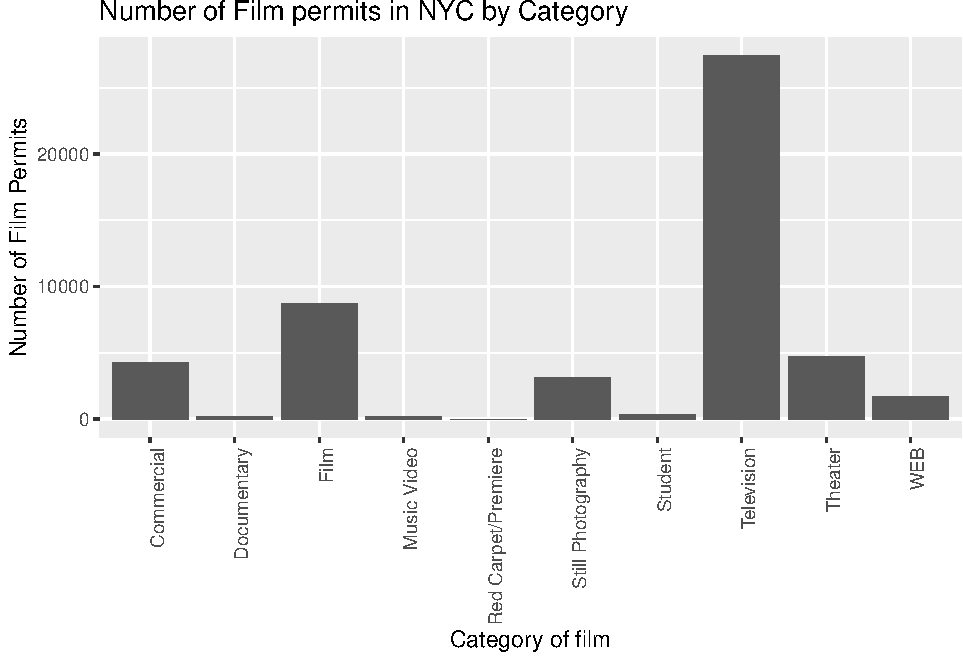
\includegraphics{Programming_Crump_files/figure-latex/unnamed-chunk-11-1.pdf}

Whenever you have a variable with multiple numbers, you can always plot
it, just like in the above example. Remember the variable
\emph{my\_numbers} contains 100 numbers. This means there are 100 slots
in the variable. Each slot has an \emph{index} value. The index value
for the first slot is 1, the index value for the second slot is 2, and
so on. The x-axis (the bottom line in the graph) shows the index value
from 1 to 100. Remember also, that each slot contains the number 43. The
y-axis (the vertical line in the graph) shows a range of numbers. The
dots in the graph represent the value inside each slot of the variable.
Because each slot contains the value 43, we see all 100 dots, all in a
line, all positioned at 43 with respect to the y-axis.

Let's plot some of the other variables we made.

\begin{Shaded}
\begin{Highlighting}[]
\KeywordTok{plot}\NormalTok{(my_sequence)}
\end{Highlighting}
\end{Shaded}

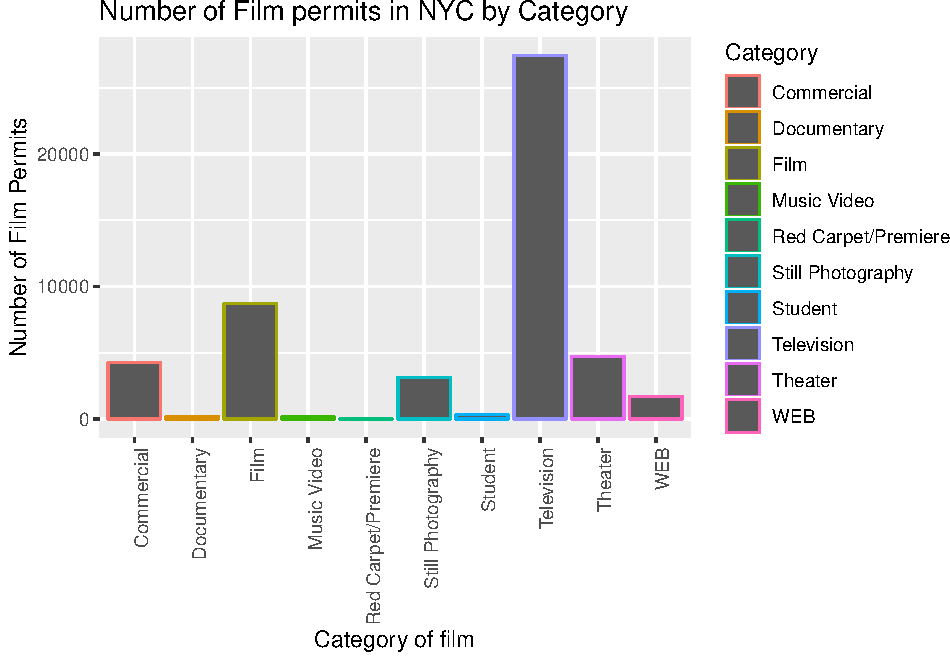
\includegraphics{Programming_Crump_files/figure-latex/unnamed-chunk-12-1.pdf}

The variable \emph{my\_sequence} contains the numbers 23 to 56, going up
by one. We see in the plot, the first number (on the x-axis) is a 23 on
the y-axis. As we go across the x-axis, the numbers go up by one until
we get to 56. We see a straight diagonal line.

\begin{Shaded}
\begin{Highlighting}[]
\KeywordTok{plot}\NormalTok{(my_randoms)}
\end{Highlighting}
\end{Shaded}

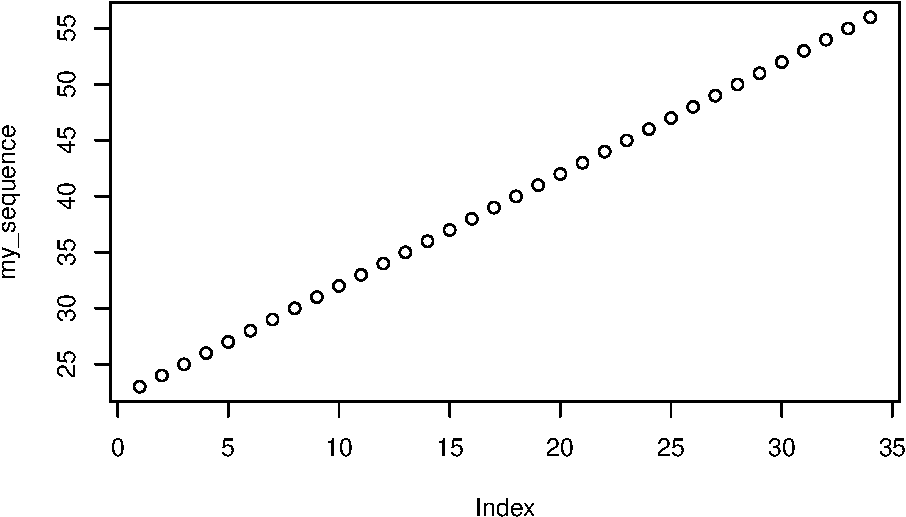
\includegraphics{Programming_Crump_files/figure-latex/unnamed-chunk-13-1.pdf}

The variable \emph{my\_randoms} contains 100 random numbers between 0
and 1. The plot shows dots all over the place between 0 and 1 on the
y-axis.

\begin{Shaded}
\begin{Highlighting}[]
\KeywordTok{plot}\NormalTok{(my_normal)}
\end{Highlighting}
\end{Shaded}

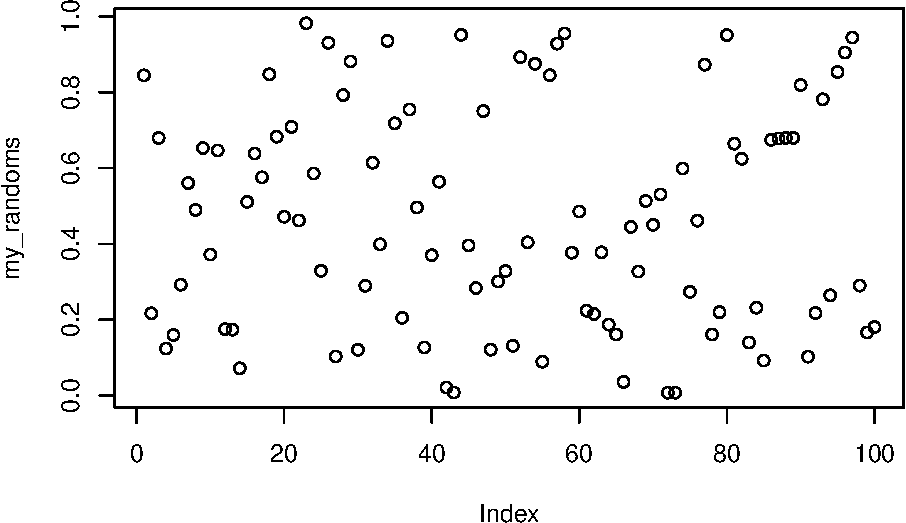
\includegraphics{Programming_Crump_files/figure-latex/unnamed-chunk-14-1.pdf}

The variable \emph{my\_normal} contains 100 numbers sample from a normal
distribution with a mean of 10, and a standard deviation of 20. Roughly,
most of the numbers should be close to 10, some of the numbers will be
greater and smaller than 10. But, as the numbers move away from 10 in
either direction, really small or really big numbers should occur less
and less frequently. We can sort of see this in the plot. For example,
you might notice that most the numbers are near the horizontal middle of
the graph, near the 10 on the y-axis, and less of the numbers are near
the top or bottom of the graph.

\subsubsection{Histograms}\label{histograms}

Histograms are used to visually summarize a set of numbers. In
particular, histograms split a set of numbers into bins, and then show
how many numbers fall within each bin. Each bin represents a pre-defined
range.

Let's create a set of numbers made up from 1s, 2s, and 3s. Let's say we
have ten 1s, twenty 2s, and 30 3s.

\begin{Shaded}
\begin{Highlighting}[]
\NormalTok{my_set <-}\StringTok{ }\KeywordTok{c}\NormalTok{(}\KeywordTok{rep}\NormalTok{(}\DecValTok{1}\NormalTok{,}\DecValTok{10}\NormalTok{),}\KeywordTok{rep}\NormalTok{(}\DecValTok{2}\NormalTok{,}\DecValTok{20}\NormalTok{),}\KeywordTok{rep}\NormalTok{(}\DecValTok{3}\NormalTok{,}\DecValTok{30}\NormalTok{))}
\end{Highlighting}
\end{Shaded}

The above line of code uses two R functions, rep(), and c(). We already
know how rep works. The c() function is short for combine. So, the above
line of code, combines 10 1s, 20 2s and 30 3s, all into one variable.
The contents of the variable looks like this:

\begin{Shaded}
\begin{Highlighting}[]
\NormalTok{my_set}
\end{Highlighting}
\end{Shaded}

\begin{verbatim}
##  [1] 1 1 1 1 1 1 1 1 1 1 2 2 2 2 2 2 2 2 2 2 2 2 2 2 2 2 2 2 2 2 3 3 3 3 3
## [36] 3 3 3 3 3 3 3 3 3 3 3 3 3 3 3 3 3 3 3 3 3 3 3 3 3
\end{verbatim}

Because, we made this variable, we already know what is inside it. Let's
make a histogram of the variable, to see what that looks like:

\begin{Shaded}
\begin{Highlighting}[]
\KeywordTok{hist}\NormalTok{(my_set)}
\end{Highlighting}
\end{Shaded}

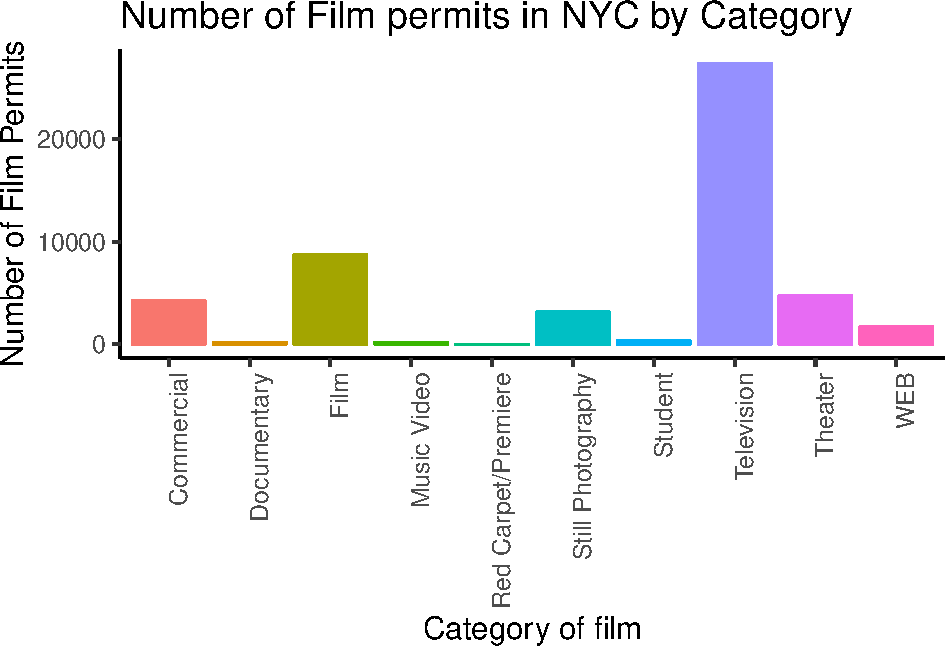
\includegraphics{Programming_Crump_files/figure-latex/unnamed-chunk-17-1.pdf}

The histogram is a bar graph. The height of each bar represents a count,
or the frequency of how many numbers fall inside each bin. The x-axis
shows the bin ranges. If you do not specify the bin ranges, then R will
make a reasonable guess for you. In this case, R set the bin ranges in
steps of .5. For example, 1-1.5, 1.5-2, 2-2.5, 2.5-3. R uses the word
\emph{breaks} to refer to bins. And, when you plot a histogram, you can
set your own breaks, or bin ranges.

\begin{Shaded}
\begin{Highlighting}[]
\KeywordTok{hist}\NormalTok{(my_set, }\DataTypeTok{breaks=}\KeywordTok{c}\NormalTok{(}\DecValTok{0}\NormalTok{,}\DecValTok{1}\NormalTok{,}\DecValTok{2}\NormalTok{,}\DecValTok{3}\NormalTok{,}\DecValTok{4}\NormalTok{))}
\end{Highlighting}
\end{Shaded}

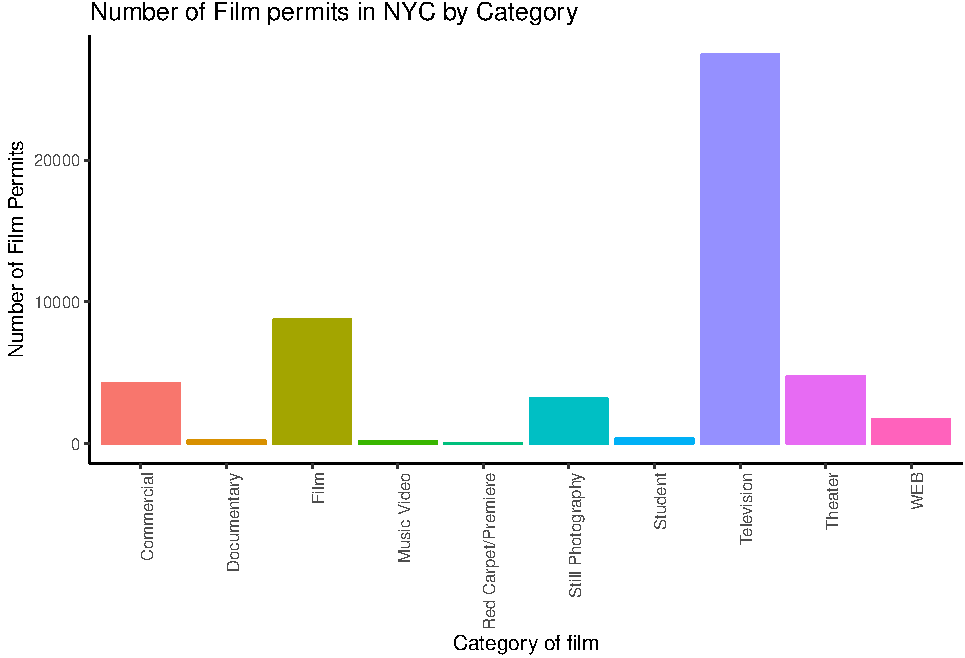
\includegraphics{Programming_Crump_files/figure-latex/unnamed-chunk-18-1.pdf}

Let's spend a moment interpreting this new histogram. The first bar is
between 0 and 1 on the x-axis, and has a value of 10 on the y-axis. This
means that there are 10 numbers inside the my\_set variable that have a
value between 0 and 1; specifically, a value greater than zero up to and
equalling 1. The second bar is between 1 and 2 on the x-axis, and has a
value of 20 on the y-axis. So, there are 20 numbers in the variable with
a value greater than 1 up to and equalling 2. Finally, the third bar
shows there are 30 numbers in the range greater than 2, up to equalling
3. We can also see there are no numbers smaller than 0, or greater than
4.

\subsubsection{What are histograms useful
for?}\label{what-are-histograms-useful-for}

A primary purpose of histograms is to get a quick look at the range and
frequency of a set of numbers. In particular, when the bars are of
different sizes, we can know that some values occur more than others.

What should a histogram look like for a set of values whose numbers all
occur randomly, and equally frequently? By this definition, we are
saying that all numbers, within all ranges, occur equally often. For
example, imagine we created a set of 10,000 numbers, and chose those
numbers from between 1 and 10, such that any number between 1 and 10
occurs with the same frequency as all other numbers. We can use the
random number generator and histogram to find out:

\begin{Shaded}
\begin{Highlighting}[]
\NormalTok{some_random_numbers <-}\StringTok{ }\KeywordTok{runif}\NormalTok{(}\DecValTok{10000}\NormalTok{,}\DecValTok{1}\NormalTok{,}\DecValTok{10}\NormalTok{)}
\KeywordTok{hist}\NormalTok{(some_random_numbers,}\DataTypeTok{breaks=}\KeywordTok{seq}\NormalTok{(}\DecValTok{0}\NormalTok{,}\DecValTok{11}\NormalTok{,}\DecValTok{1}\NormalTok{))}
\end{Highlighting}
\end{Shaded}

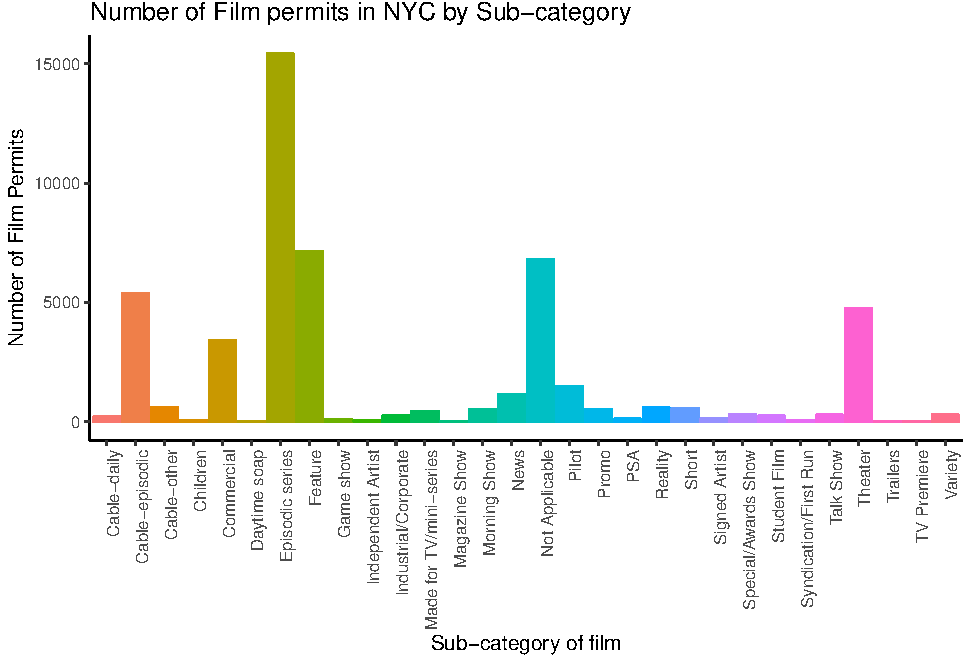
\includegraphics{Programming_Crump_files/figure-latex/unnamed-chunk-19-1.pdf}

\begin{Shaded}
\begin{Highlighting}[]
\CommentTok{#notice I set the breaks using the seq() function}
\end{Highlighting}
\end{Shaded}

We see that heights of the bars are all close to the same number. This
is good, because each number between 1 to 10 should have had an equal
chance of being selected. However, notice the bars are not exactly the
same height. This shows that the random number generator did actually
generate each number with equal frequency.

What about sets of numbers where some kinds of numbers occur more than
others? Here, we would expect higher bars for ranges containing many
values, and smaller numbers for ranges containing fewer values.

Let's plot histogram for a normal distribution and see what it looks
like. We will set the mean to 100, and the standard deviation to 20, and
we ask R to generate 10000 numbers from this distribution.

\begin{Shaded}
\begin{Highlighting}[]
\NormalTok{normal_sample <-}\StringTok{ }\KeywordTok{rnorm}\NormalTok{(}\DecValTok{10000}\NormalTok{,}\DecValTok{100}\NormalTok{,}\DecValTok{20}\NormalTok{)}
\KeywordTok{hist}\NormalTok{(normal_sample)}
\end{Highlighting}
\end{Shaded}

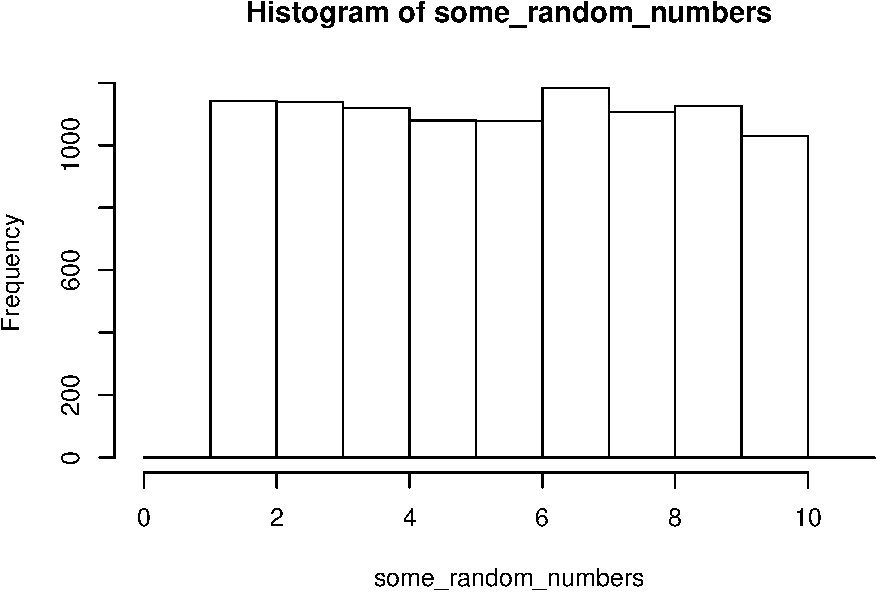
\includegraphics{Programming_Crump_files/figure-latex/unnamed-chunk-20-1.pdf}
The histogram shows that the highest bars are in the middle, near the
100 mark. So, numbers near 100 occured most frequently in our set. What
happens to the heights of the bars on either side of the histogram? The
bars are decreasing in height as they move away from the middle in both
directions. So, as numbers move away from 100, they occur less and less
frequently. For example, we don't see any bars in the range of 500 or
1000. This means that no values that high were in our set of numbers.
From the histogram, we can clearly see that our set hardly had any
numbers greater than 150, or less than 50. Or, in other words, most of
the numbers were between 50 and 150.

\section{Excel}\label{excel}

\section{SPSS}\label{spss}

\section{Matlab}\label{matlab}

\chapter{Lab 2: Descriptive
Statistics}\label{lab-2-descriptive-statistics}

{ Some inspiring quote ---Inspiring Person }

\section{Outline of Problem to solve}\label{outline-of-problem-to-solve}

Stuff we need to say in general

\subsection{important things}\label{important-things}

Other things to say

\section{R}\label{r-2}

How to do it in R

\section{Excel}\label{excel-1}

How to do it in Excel

\section{SPSS}\label{spss-1}

How to do it in SPSS

\section{Matlab}\label{matlab-1}

How to do it in Matlab

\chapter{Lab 3: Correlation}\label{lab-3-correlation}

{ Some inspiring quote ---Inspiring Person }

\section{Outline of Problem to
solve}\label{outline-of-problem-to-solve-1}

Stuff we need to say in general

\subsection{important things}\label{important-things-1}

Other things to say

\section{R}\label{r-3}

How to do it in R

\section{Excel}\label{excel-2}

How to do it in Excel

\section{SPSS}\label{spss-2}

How to do it in SPSS

\section{Matlab}\label{matlab-2}

How to do it in Matlab

\chapter{Lab 5: Normal Distribution \& Central Limit
Theorem}\label{lab-5-normal-distribution-central-limit-theorem}

{ Some inspiring quote ---Inspiring Person }

\section{Outline of Problem to
solve}\label{outline-of-problem-to-solve-2}

Stuff we need to say in general

\subsection{important things}\label{important-things-2}

Other things to say

\section{R}\label{r-4}

How to do it in R

\section{Excel}\label{excel-3}

How to do it in Excel

\section{SPSS}\label{spss-3}

How to do it in SPSS

\section{Matlab}\label{matlab-3}

How to do it in Matlab

\chapter{Lab 6: Fundamentals of Hypothesis
Testing}\label{lab-6-fundamentals-of-hypothesis-testing}

{ Some inspiring quote ---Inspiring Person }

\section{Outline of Problem to
solve}\label{outline-of-problem-to-solve-3}

Stuff we need to say in general

\subsection{important things}\label{important-things-3}

Other things to say

\section{R}\label{r-5}

How to do it in R

\section{Excel}\label{excel-4}

How to do it in Excel

\section{SPSS}\label{spss-4}

How to do it in SPSS

\section{Matlab}\label{matlab-4}

How to do it in Matlab

\chapter{Lab 8: t-Test (one-sample, paired
sample)}\label{lab-8-t-test-one-sample-paired-sample}

{ Some inspiring quote ---Inspiring Person }

\section{Outline of Problem to
solve}\label{outline-of-problem-to-solve-4}

Stuff we need to say in general

\subsection{important things}\label{important-things-4}

Other things to say

\section{R}\label{r-6}

How to do it in R

\section{Excel}\label{excel-5}

How to do it in Excel

\section{SPSS}\label{spss-5}

How to do it in SPSS

\section{Matlab}\label{matlab-5}

How to do it in Matlab

\chapter{Lab 9: t-test (Independent
Sample)}\label{lab-9-t-test-independent-sample}

{ Some inspiring quote ---Inspiring Person }

\section{Outline of Problem to
solve}\label{outline-of-problem-to-solve-5}

Stuff we need to say in general

\subsection{important things}\label{important-things-5}

Other things to say

\section{R}\label{r-7}

How to do it in R

\section{Excel}\label{excel-6}

How to do it in Excel

\section{SPSS}\label{spss-6}

How to do it in SPSS

\section{Matlab}\label{matlab-6}

How to do it in Matlab

\chapter{Lab 10: One-way ANOVA}\label{lab-10-one-way-anova}

{ Some inspiring quote ---Inspiring Person }

\section{Outline of Problem to
solve}\label{outline-of-problem-to-solve-6}

Stuff we need to say in general

\subsection{important things}\label{important-things-6}

Other things to say

\section{R}\label{r-8}

How to do it in R

\section{Excel}\label{excel-7}

How to do it in Excel

\section{SPSS}\label{spss-7}

How to do it in SPSS

\section{Matlab}\label{matlab-7}

How to do it in Matlab

\chapter{Lab 10: One-way ANOVA}\label{lab-10-one-way-anova-1}

{ Some inspiring quote ---Inspiring Person }

\section{Outline of Problem to
solve}\label{outline-of-problem-to-solve-7}

Stuff we need to say in general

\subsection{important things}\label{important-things-7}

Other things to say

\section{R}\label{r-9}

How to do it in R

\section{Excel}\label{excel-8}

How to do it in Excel

\section{SPSS}\label{spss-8}

How to do it in SPSS

\section{Matlab}\label{matlab-8}

How to do it in Matlab

\chapter{Lab 11: Factorial ANOVA}\label{lab-11-factorial-anova}

{ Some inspiring quote ---Inspiring Person }

\section{Outline of Problem to
solve}\label{outline-of-problem-to-solve-8}

Stuff we need to say in general

\subsection{important things}\label{important-things-8}

Other things to say

\section{R}\label{r-10}

How to do it in R

\section{Excel}\label{excel-9}

How to do it in Excel

\section{SPSS}\label{spss-9}

How to do it in SPSS

\section{Matlab}\label{matlab-9}

How to do it in Matlab

\chapter{Lab 12: Repeated Measures Factorial
ANOVA}\label{lab-12-repeated-measures-factorial-anova}

{ Some inspiring quote ---Inspiring Person }

\section{Outline of Problem to
solve}\label{outline-of-problem-to-solve-9}

Stuff we need to say in general

\subsection{important things}\label{important-things-9}

Other things to say

\section{R}\label{r-11}

How to do it in R

\section{Excel}\label{excel-10}

How to do it in Excel

\section{SPSS}\label{spss-10}

How to do it in SPSS

\section{Matlab}\label{matlab-10}

How to do it in Matlab

\bibliography{book.bib,packages.bib,MyLibrary.bib}


\end{document}
